\documentclass[aspectratio=169,11pt]{beamer}

\usepackage[T1]{fontenc}
\usepackage[sfdefault,semibold,lining]{sourcesanspro}
\usefonttheme[onlymath]{serif}
\usepackage{amsmath,amssymb,bm}
\usepackage{booktabs}
\usepackage{tikz}
\usetikzlibrary{arrows.meta,positioning,calc}
\usepackage[most]{tcolorbox}
\usepackage{fontawesome5}
\usepackage{appendixnumberbeamer}
\graphicspath{{../results/figures/}}

% ---- fill in team member names ------------------------------------------
\newcommand{\memberA}{Member A}
\newcommand{\memberB}{Member B}
\newcommand{\memberC}{Member C}
\newcommand{\memberD}{Member D}
% -------------------------------------------------------------------------

% ============================== theme ====================================
\definecolor{ink}{HTML}{1E2A3A}
\definecolor{body}{HTML}{2B2F36}
\definecolor{accent}{HTML}{E4572E}
\definecolor{second}{HTML}{1F7A6D}
\definecolor{muted}{HTML}{8A93A3}
\definecolor{hair}{HTML}{D9DDE3}

\setbeamercolor{normal text}{fg=body,bg=white}
\setbeamercolor{structure}{fg=ink}
\setbeamercolor{alerted text}{fg=accent}
\setbeamercolor{frametitle}{fg=ink}
\setbeamercolor{footline}{fg=muted}
\setbeamercolor{section in head/foot}{fg=accent}
\setbeamercolor{description item}{fg=second}

\setbeamerfont{frametitle}{size=\fontsize{17}{20}\selectfont,series=\bfseries}
\setbeamerfont{eyebrow}{size=\scriptsize,series=\bfseries}
\setbeamerfont{footline}{size=\tiny}
\setbeamerfont{section in head/foot}{size=\tiny}
\setbeamerfont{block title}{size=\small,series=\bfseries}

\setbeamersize{text margin left=1.1cm,text margin right=1.1cm}
\setbeamertemplate{navigation symbols}{}
\setbeamertemplate{headline}{}
\setbeamertemplate{section in head/foot shaded}[default][35]

\setbeamertemplate{itemize item}{\raisebox{0.28ex}{\color{accent}\rule{0.4em}{0.4em}}}
\setbeamertemplate{itemize subitem}{\color{muted}\textendash}
\setbeamertemplate{enumerate item}{\color{accent}\bfseries\insertenumlabel}
\setbeamertemplate{description item}{\color{second}\bfseries\insertdescriptionitem}

\newcommand{\twodigit}[1]{\ifnum#1<10 0\fi\number#1}
\newcommand{\sectionspeaker}{\ifcase\value{section}\or\memberA\or\memberB\or\memberC\or\memberD\fi}
\newif\ifbackup

\makeatletter
% section label on the left, speaker tag on the right, then the title
\setbeamertemplate{frametitle}{%
  \vspace*{0.15cm}%
  \begin{minipage}[t]{\linewidth}%
    {\usebeamerfont{eyebrow}%
     \ifbackup\textcolor{muted}{BACKUP}%
     \else\ifnum\value{section}>0\textcolor{accent}{\twodigit{\value{section}}\enspace\rule[0.3ex]{1.2em}{0.6pt}\enspace\insertsectionhead}\fi\fi
     \hfill
     \ifx\insertframesubtitle\@empty\else
       \tikz[baseline=(t.base)]\node[fill=second!10,text=second,rounded corners=6pt,inner xsep=6pt,inner ysep=2.5pt](t){\faMicrophone\enspace\insertframesubtitle};%
     \fi\par}%
    \vspace{0.25em}%
    {\usebeamerfont{frametitle}\usebeamercolor[fg]{frametitle}\insertframetitle\par}%
  \end{minipage}%
  \vspace{0.1cm}%
}
\makeatother

\setbeamertemplate{footline}{%
  \hspace*{1.1cm}%
  \begin{minipage}[b][0.55cm][t]{\dimexpr\paperwidth-2.2cm\relax}%
    {\color{hair}\rule{\linewidth}{0.5pt}}\par\vspace{3pt}%
    \usebeamerfont{footline}\usebeamercolor[fg]{footline}%
    LSTD($\lambda$)\enspace\textperiodcentered\enspace Boyan, ICML 1999%
    \hfill\insertsectionnavigationhorizontal{0.6\linewidth}{}{}\hfill
    {\color{ink}\bfseries\insertframenumber}\,/\,\inserttotalframenumber
  \end{minipage}%
}

\tcbset{flatbox/.style={enhanced,frame hidden,arc=0pt,outer arc=0pt,boxsep=0pt,
  left=8pt,right=8pt,top=5pt,bottom=5pt,before skip=4pt,after skip=4pt,before upper=\raggedright}}
\setbeamertemplate{block begin}{%
  \begin{tcolorbox}[flatbox,colback=second!6,borderline west={2.5pt}{0pt}{second}]%
  {\usebeamerfont{block title}\color{second}\insertblocktitle\par}\vspace{0.3em}}
\setbeamertemplate{block end}{\end{tcolorbox}}

\newtcolorbox{keyidea}{flatbox,colback=accent!7,borderline west={3pt}{0pt}{accent},
  left=10pt,top=7pt,bottom=7pt,fontupper=\large\color{ink}}
\newcommand{\stat}[2]{%
  \begin{tcolorbox}[flatbox,colback=white,borderline west={2.5pt}{0pt}{accent},top=0pt,bottom=0pt,before skip=0pt,after skip=5pt]
    {\fontsize{16}{18}\selectfont\bfseries\color{accent}#1}\par
    {\scriptsize\color{body}#2}
  \end{tcolorbox}}

\newcommand{\darkbg}{\fill[ink] (current page.south west) rectangle (current page.north east);}

\AtBeginSection[]{%
  \begin{frame}[plain,noframenumbering]
  \begin{tikzpicture}[remember picture,overlay]
    \darkbg
    \node[anchor=south west,inner sep=0pt,text=accent,font=\fontsize{72}{72}\selectfont\bfseries]
      at ([xshift=1.0cm,yshift=0.15cm]current page.west) {\twodigit{\value{section}}};
    \node[anchor=north west,inner sep=0pt,text=white,font=\fontsize{26}{30}\selectfont\bfseries,text width=12cm]
      at ([xshift=1.1cm,yshift=-0.35cm]current page.west) {\insertsectionhead};
    \node[anchor=north west,inner sep=0pt,text=white!60!ink,font=\small]
      at ([xshift=1.1cm,yshift=-1.6cm]current page.west) {\faMicrophone\enspace\sectionspeaker};
    \foreach \k in {1,...,4} {
      \ifnum\k=\value{section}\def\barcol{accent}\else\def\barcol{white!25!ink}\fi
      \fill[\barcol] ([xshift=1.1cm+(\k-1)*1.0cm,yshift=1.0cm]current page.south west) rectangle ++(0.8cm,0.08cm);
    }
  \end{tikzpicture}
  \end{frame}}
% =========================================================================

\newcommand{\speaker}[1]{\framesubtitle{#1}}
\newcommand{\hl}[1]{\textcolor{accent}{\textbf{#1}}}
\newcommand{\vphi}{\bm{\phi}}
\newcommand{\vz}{\mathbf{z}}
\newcommand{\vth}{\bm{\theta}}
\tikzset{st/.style={circle,draw=ink,thick,fill=second!8,minimum size=7mm,inner sep=0pt,font=\small},
         arr/.style={-{Stealth[length=2mm]},thick,draw=ink!80}}

\title{Least-Squares Temporal Difference Learning}
\author{\memberA, \memberB, \memberC, \memberD}
\date{November 2026}

\begin{document}

% =========================================================================
\begin{frame}[plain,noframenumbering]
  \begin{tikzpicture}[remember picture,overlay]
    \darkbg
    % motif: the 13-state Boyan chain bending around the bottom-right corner
    \begin{scope}[shift={(current page.south east)}]
      \foreach \i in {0,...,12} {\coordinate (c\i) at ({96+\i*6}:5.6cm);}
      \foreach \i [evaluate=\i as \j using int(\i+1)] in {0,...,11}
        \draw[white!22!ink,line width=0.8pt] (c\i) -- (c\j);
      \foreach \i [evaluate=\i as \j using int(\i+2)] in {0,...,10}
        \draw[white!14!ink,line width=0.6pt] (c\i) to[bend left=40] (c\j);
      \foreach \i in {0,...,12} {
        \pgfmathtruncatemacro{\mix}{100-\i*7}
        \fill[accent!\mix!second] (c\i) circle (0.16cm);
      }
      \draw[white!70!ink,line width=0.6pt] (c12) circle (0.26cm);
    \end{scope}
    \node[anchor=north west,inner sep=0pt,text=accent,font=\scriptsize\bfseries]
      at ([xshift=1.1cm,yshift=-0.9cm]current page.north west)
      {E1 277 \textperiodcentered{} COURSE PROJECT \textperiodcentered{} PAPER \#22};
    \node[anchor=north west,inner sep=0pt,text=white,text width=10cm,align=left,
          font=\fontsize{28}{32}\selectfont\bfseries]
      at ([xshift=1.1cm,yshift=-1.6cm]current page.north west)
      {Least-Squares\\Temporal Difference\\Learning};
    \fill[accent] ([xshift=1.1cm,yshift=-5.25cm]current page.north west) rectangle ++(1.4cm,0.09cm);
    \node[anchor=north west,inner sep=0pt,text=white!72!ink,text width=9cm,align=left]
      at ([xshift=1.1cm,yshift=-5.6cm]current page.north west)
      {Reimplementing Boyan (ICML 1999)\\and a ridge-regularised extension};
    \node[anchor=south west,inner sep=0pt,align=left]
      at ([xshift=1.1cm,yshift=0.75cm]current page.south west)
      {\color{white}\small\bfseries \memberA\quad\textperiodcentered\quad\memberB\quad\textperiodcentered\quad\memberC\quad\textperiodcentered\quad\memberD\\[3pt]
       \color{white!55!ink}\scriptsize E1 277 Reinforcement Learning\enspace\textperiodcentered\enspace November 2026};
  \end{tikzpicture}
\end{frame}

\begin{frame}{What we did}
  \begin{columns}[T]
    \column{0.55\textwidth}
    \textbf{One-line summary.} TD($\lambda$) solves a linear system by slow, noisy gradient steps.
    LSTD($\lambda$) estimates that system from data and \hl{solves it directly}: same answer, less data, no step size.
    \vspace{0.6em}

    \textbf{Talk outline}
    \begin{enumerate}
      \item Motivation \& setup \hfill \memberA
      \item TD($\lambda$) and its weaknesses \hfill \memberB
      \item The LSTD($\lambda$) algorithm \hfill \memberC
      \item Experiments \& novelty \hfill \memberD
    \end{enumerate}
    \column{0.42\textwidth}
    \small
    \begin{tabular}{@{}p{0.41\linewidth}p{0.53\linewidth}@{}}
      \toprule
      \textbf{Course task} & \textbf{Our work} \\
      \midrule
      Understand algorithm & Derivation + paper's equivalences proved as unit tests \\
      Run authors' code & None public (1999) $\Rightarrow$ full reimplementation, matches paper Figs.~5--6 \\
      Change settings & $\lambda$, 12 TD step sizes, feature dim.\ $d$ \\
      New environment & 19-state random walk, weak features \\
      Improvement & Ridge LSTD for very few trajectories \\
      \bottomrule
    \end{tabular}
  \end{columns}
\end{frame}

% =========================================================================
\section{Motivation \& setup}

\begin{frame}{Policy evaluation}
  \speaker{\memberA}
  \begin{itemize}
    \item Fixed policy $\pi$ in an MDP $\Rightarrow$ a Markov chain with rewards.
    \item \textbf{Value function}: expected total future reward from each state
      \[ V^\pi(s) = \mathbb{E}\Big[\textstyle\sum_{t\ge 0} \gamma^t r_t \;\Big|\; s_0 = s\Big] \]
    \item Inner loop of policy iteration, actor--critic, STAGE, \ldots
    \item If the transition matrix $P$ is known, it is just a linear system (Bellman equation):
      \[ V = r + \gamma P V \]
    \item \hl{In practice:} (1) $P$ is unknown --- we only see sampled trajectories;
      (2) too many states to store a table.
  \end{itemize}
\end{frame}

\begin{frame}{Linear function approximation}
  \speaker{\memberA}
  \begin{itemize}
    \item Describe each state by $K$ features $\vphi(s)\in\mathbb{R}^K$ and learn only $K$ weights:
      \[ \hat V(s) = \vphi(s)^\top \vth \]
    \item Covers lookup tables, state aggregation, tile coding / CMACs, RBFs, polynomials.
    \item \textbf{Data:} trajectories of transitions $(s_t,\, r_t,\, s_{t+1})$ until termination.
    \item \textbf{Goal:} find $\vth$ such that $\hat V \approx V^\pi$, using as few trajectories as possible.
    \item \textbf{Metric (paper):} RMS error over all states
      \[ \mathrm{RMSE} = \sqrt{\tfrac{1}{|S|}\textstyle\sum_s \big(\vphi(s)^\top\vth - V^\pi(s)\big)^2} \]
  \end{itemize}
\end{frame}

\begin{frame}{Monte Carlo vs.\ TD: the intuition}
  \speaker{\memberA}
  \begin{center}
    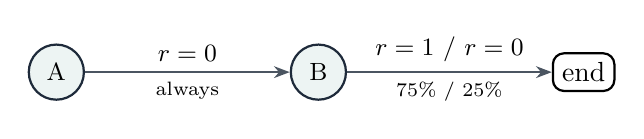
\begin{tikzpicture}
      \node[st] (A) {A};
      \node[st, right=2.6cm of A] (B) {B};
      \node[draw,thick,rounded corners, right=2.6cm of B] (E) {end};
      \draw[arr] (A) -- node[above]{\small $r=0$} node[below]{\scriptsize always} (B);
      \draw[arr] (B) -- node[above]{\small $r=1$ / $r=0$} node[below]{\scriptsize 75\% / 25\%} (E);
    \end{tikzpicture}
  \end{center}
  \begin{columns}[T]
    \column{0.48\textwidth}
    \small
    \textbf{Data:} 8 episodes. One starts at A and is unlucky (A$\to$B$\to$0). Seven start at B: six pay 1, one pays 0.
    \vspace{0.4em}

    \textbf{MC}: target = actual return.\\ ``From A I once got 0'' $\Rightarrow \hat V(A)=0$.\\[0.3em]
    \textbf{TD}: target = $r + \hat V(\text{next})$.\\ ``A gives 0 then B, and B averages 0.75'' $\Rightarrow \hat V(A)=0.75$.
    \column{0.48\textwidth}
    \small
    \begin{tabular}{lccc}
      \toprule
      & True & MC & TD \\
      \midrule
      $V(B)$ & 0.75 & 0.75 & 0.75 \\
      $V(A)$ & 0.75 & \hl{0} & \hl{0.75} \\
      \bottomrule
    \end{tabular}
    \vspace{0.5em}

    MC: unbiased, \emph{high variance}.\\
    TD: \emph{bootstraps} from its own estimate; low variance, biased while estimates are wrong.
  \end{columns}
\end{frame}

\begin{frame}{Test domain: the Boyan chain (paper Fig.~4)}
  \speaker{\memberA}
  \begin{center}
    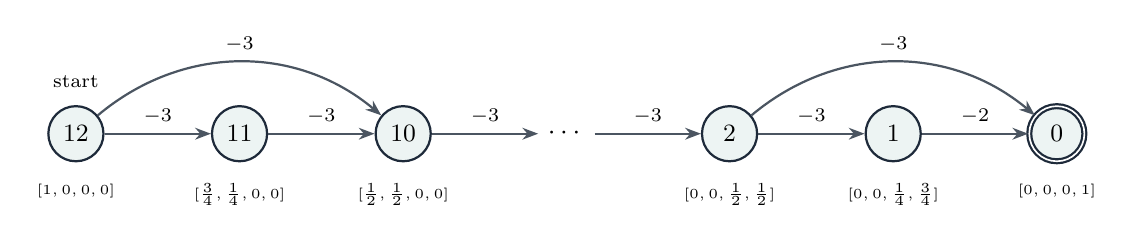
\begin{tikzpicture}[node distance=1.35cm]
      \node[st] (s12) {12};
      \node[st, right=of s12] (s11) {11};
      \node[st, right=of s11] (s10) {10};
      \node[right=of s10] (dots) {$\cdots$};
      \node[st, right=of dots] (s2) {2};
      \node[st, right=of s2] (s1) {1};
      \node[st, double, right=of s1] (s0) {0};
      \foreach \a/\b in {s12/s11, s11/s10, s10/dots, dots/s2, s2/s1}
        \draw[arr] (\a) -- node[above]{\scriptsize $-3$} (\b);
      \draw[arr] (s1) -- node[above]{\scriptsize $-2$} (s0);
      \draw[arr] (s12) to[bend left=40] node[above]{\scriptsize $-3$} (s10);
      \draw[arr] (s2) to[bend left=40] node[above]{\scriptsize $-3$} (s0);
      \node[above=0.1cm of s12] {\scriptsize start};
      \node[below=0.15cm of s12, font=\tiny] {$[1,0,0,0]$};
      \node[below=0.15cm of s11, font=\tiny] {$[\frac34,\frac14,0,0]$};
      \node[below=0.15cm of s10, font=\tiny] {$[\frac12,\frac12,0,0]$};
      \node[below=0.15cm of s2, font=\tiny] {$[0,0,\frac12,\frac12]$};
      \node[below=0.15cm of s1, font=\tiny] {$[0,0,\frac14,\frac34]$};
      \node[below=0.15cm of s0, font=\tiny] {$[0,0,0,1]$};
    \end{tikzpicture}
  \end{center}
  \begin{itemize}
    \item 13 states, start at 12, state 0 terminal, $\gamma = 1$. From $s\ge2$: go to $s{-}1$ or $s{-}2$ (prob.\ $\tfrac12$ each), reward $-3$.
    \item $K=4$ features: anchors at 12, 8, 4, 0; linear interpolation in between.
    \item True values $V^\pi(s) = -2s$ are \hl{exactly representable}: $\vth^* = (-24,-16,-8,0)$.
    \item Every constant above checked against the paper and covered by unit tests.
  \end{itemize}
\end{frame}

% =========================================================================
\section{TD($\lambda$)}

\begin{frame}{From TD(0) to TD($\lambda$)}
  \speaker{\memberB}
  \textbf{TD(0)}: nudge $\vth$ toward a one-step target
  \[ \delta_t = r_t + \gamma\,\vphi(s_{t+1})^\top\vth - \vphi(s_t)^\top\vth, \qquad
     \vth \leftarrow \vth + \alpha\,\delta_t\,\vphi(s_t) \]
  \textbf{TD($\lambda$)}: credit each TD error to \emph{all recent} states via an eligibility trace
  \[ \vz_t = \gamma\lambda\,\vz_{t-1} + \vphi(s_t), \qquad \vth \leftarrow \vth + \alpha\,\delta_t\,\vz_t \]
  \begin{columns}[T]
    \column{0.5\textwidth}
    \begin{itemize}
      \item $\lambda = 0$: one-step TD (low variance, biased)
      \item $\lambda = 1$: Monte Carlo (unbiased, high variance)
      \item In between: trades bias for variance
    \end{itemize}
    \column{0.47\textwidth}
    \begin{itemize}
      \item $\vz_t$ propagates reward backwards \emph{without storing the trajectory}
      \item Cost: $O(K)$ per step
    \end{itemize}
  \end{columns}
\end{frame}

\begin{frame}{TD($\lambda$) in the paper (Fig.~1) and step sizes}
  \speaker{\memberB}
  \begin{columns}[T]
    \column{0.5\textwidth}
    \begin{block}{TD($\lambda$), offline (paper Fig.~1)}
      \small
      for trajectory $n = 1, 2, \ldots$\\
      \quad $\Delta \leftarrow 0$, \ $\vz \leftarrow \vphi(s_0)$\\
      \quad for each step $t$:\\
      \qquad $\Delta \leftarrow \Delta + \vz\,\big(r_t + (\vphi_{t+1} - \vphi_t)^\top\vth\big)$\\
      \qquad $\vz \leftarrow \lambda\vz + \vphi_{t+1}$\\
      \quad $\vth \leftarrow \vth + \alpha_n \Delta$
    \end{block}
    \small $\vphi(\text{end}) = 0$; $\vth$ is fixed within a trajectory.
    \column{0.47\textwidth}
    \textbf{Step-size schedule (paper Eq.~8)}
    \[ \alpha_n = a_0\,\frac{n_0+1}{n_0+n} \]
    \begin{itemize}
      \item $a_0 \in \{0.1,\ 0.01\}$
      \item $n_0 \in \{10^2,\ 10^3,\ 10^6\}$
      \item $\Rightarrow$ 6 schedules (paper)
      \item \textbf{We add} 6 constant $\alpha \in \{0.001,\ldots,0.3\}$
      \item $\Rightarrow$ 12 TD configurations per $\lambda$
    \end{itemize}
  \end{columns}
\end{frame}

\begin{frame}{Weakness of TD: the step size}
  \speaker{\memberB}
  \begin{columns}[c]
    \column{0.58\textwidth}
    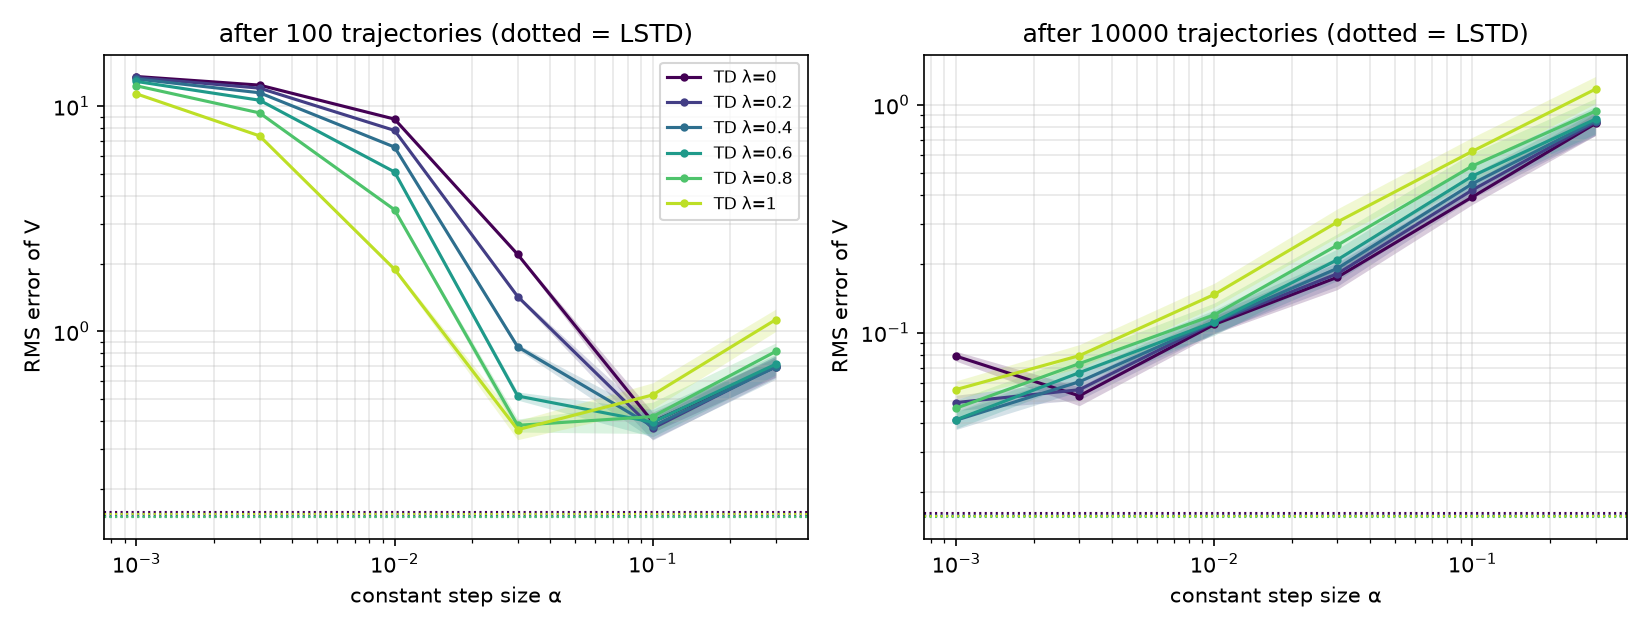
\includegraphics[width=\linewidth]{fig2_td_alpha.png}
    \column{0.40\textwidth}
    \small
    \textbf{No single $\alpha$ is good both early and late} ($\lambda=0.4$, RMSE):
    \vspace{0.3em}

    \begin{tabular}{@{}l@{\hspace{6pt}}c@{\hspace{6pt}}c@{}}
      \toprule
      & $n=100$ & $n=10^4$ \\
      \midrule
      TD $\alpha=0.3$ & 0.70 & 0.85 \\
      TD $\alpha=0.001$ & 13.2 & 0.041 \\
      TD, best sched. & 0.31 & 0.036 \\
      \textbf{LSTD} & \textbf{0.15} & \textbf{0.016} \\
      \bottomrule
    \end{tabular}
    \vspace{0.4em}

    Other weaknesses (paper): sensitive to initial $\vth$ and to feature scaling; each sample used once, then forgotten.
  \end{columns}
\end{frame}

% =========================================================================
\section{LSTD($\lambda$)}

\begin{frame}{Where does TD($\lambda$) converge?}
  \speaker{\memberC}
  \begin{itemize}
    \item Averaged over trajectories, one TD($\lambda$) pass changes $\vth$ by
      \[ \mathbb{E}[\Delta\vth] = \alpha\,(\mathbf{d} + C\vth), \quad
        \mathbf{d} = \mathbb{E}\Big[\textstyle\sum_t \vz_t r_t\Big], \quad
        C = \mathbb{E}\Big[\textstyle\sum_t \vz_t\big(\gamma\vphi_{t+1} - \vphi_t\big)^\top\Big] \]
    \item TD stops moving when
      \[ \boxed{\mathbf{d} + C\vth = 0} \]
    \item $C$ is negative definite $\Rightarrow$ unique fixed point (Tsitsiklis \& Van Roy).
    \item \hl{TD is stochastic gradient descent on a $K\times K$ linear system} --- it never writes the system down.
  \end{itemize}
  \vspace{0.2em}
  \begin{keyidea}
    \textbf{Idea:} estimate $\mathbf{d}$ and $C$ from data and solve the system directly.
  \end{keyidea}
\end{frame}

\begin{frame}{The LSTD($\lambda$) algorithm (paper Fig.~2)}
  \speaker{\memberC}
  \begin{columns}[T]
    \column{0.5\textwidth}
    \begin{block}{LSTD($\lambda$)}
      \small
      $A \leftarrow 0$, $\mathbf{b} \leftarrow 0$\\
      for each trajectory:\\
      \quad $\vz \leftarrow 0$\\
      \quad for each step $t$:\\
      \qquad $\vz \leftarrow \gamma\lambda\vz + \vphi_t$\\
      \qquad $A \leftarrow A + \vz\,(\vphi_t - \gamma\vphi_{t+1})^\top$\\
      \qquad $\mathbf{b} \leftarrow \mathbf{b} + \vz\, r_t$\\
      whenever needed: $\vth = A^{-1}\mathbf{b}$
    \end{block}
    \column{0.47\textwidth}
    \begin{itemize}
      \item After $n$ trajectories: $\mathbf{b}\approx n\mathbf{d}$, $A \approx -nC$
      \item $\Rightarrow$ $A^{-1}\mathbf{b}$ estimates TD's fixed point
      \item \hl{No step size, no initial $\vth$}
      \item Invariant to feature scaling
      \item Keeps \emph{all} data in $A$, $\mathbf{b}$
      \item Singular $A$ (too little data): paper uses SVD; we use \texttt{solve} with an SVD fallback
    \end{itemize}
  \end{columns}
\end{frame}

\begin{frame}{Three views of LSTD($\lambda$) (paper Secs.~2--3)}
  \speaker{\memberC}
  \begin{enumerate}
    \item \textbf{$\lambda=0$:} exactly Bradtke \& Barto's LSTD (1996), with a much simpler derivation.
    \item \textbf{$\lambda=1$:} least-squares regression of features onto Monte-Carlo returns,
      built \emph{incrementally} (telescoping: $A = \sum_t \vphi_t\vphi_t^\top$, $\mathbf{b} = \sum_t \vphi_t G_t$).
    \item \textbf{Model-based view:} with one feature per state, LSTD(0) accumulates
      \[ A = N - C_{\text{count}}, \quad \mathbf{b} = \mathbf{s}
        \;\Rightarrow\; \vth = (N - C_{\text{count}})^{-1}\mathbf{s}, \]
      which is exactly \hl{``count transitions, build the empirical Markov chain, solve its Bellman equations''}.
  \end{enumerate}
  \vspace{0.3em}
  \begin{block}{Corridor example, one pass over the 8 episodes}
    LSTD(0): $\hat V(A) = 0.75$ (= TD's limit).\quad
    LSTD(1): $\hat V(A) = 0$ (= MC).\quad
    TD(0) needs $\sim$2000 replays with $\alpha = 0.01$ to reach 0.75.\\
    \small All three equivalences are checked by unit tests in our repo.
  \end{block}
\end{frame}

\begin{frame}{Computational cost and recursive LSTD}
  \speaker{\memberC}
  \begin{columns}[c]
    \column{0.47\textwidth}
    \small
    \begin{tabular}{@{}lcc@{}}
      \toprule
      & per step & per solve \\
      \midrule
      TD($\lambda$) & $O(K)$ & --- \\
      LSTD($\lambda$) & $O(K^2)$ & $O(K^3)$ \\
      Recursive LSTD & $O(K^2)$ & --- \\
      \bottomrule
    \end{tabular}
    \vspace{0.6em}

    \textbf{Recursive LSTD} keeps $B = A^{-1}$ up to date (Sherman--Morrison), $\mathbf{u} = \vphi_t - \gamma\vphi_{t+1}$:
    \[ B \leftarrow B - \frac{B\vz\,\mathbf{u}^\top B}{1 + \mathbf{u}^\top B\vz} \]
    Start $B_0 = \delta I$ $\Leftrightarrow$ ridge with $\epsilon = 1/\delta$.
    \column{0.51\textwidth}
    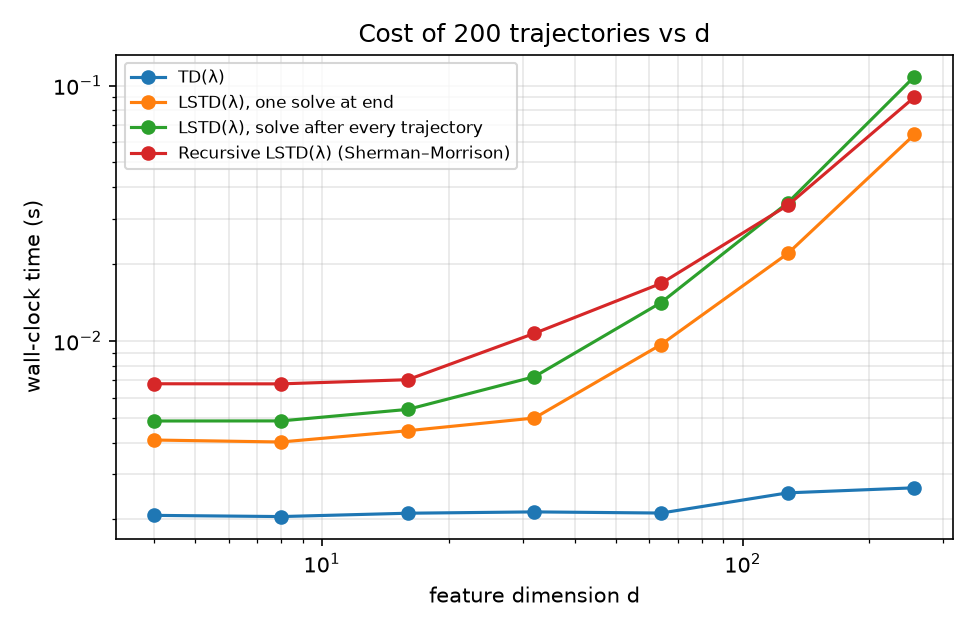
\includegraphics[width=\linewidth]{fig4_timing.png}
    \small At $d=256$: TD 2.7\,ms vs.\ LSTD 64\,ms (200 trajectories).
  \end{columns}
\end{frame}

% =========================================================================
\section{Experiments \& novelty}

\begin{frame}{Experimental setup}
  \speaker{\memberD}
  \begin{columns}[T]
    \column{0.5\textwidth}
    \textbf{Reproduction (paper Sec.~4)}
    \begin{itemize}
      \item Boyan chain, $\lambda \in \{0, 0.2, \ldots, 1\}$
      \item Up to $10^4$ trajectories
      \item LSTD vs.\ 12 TD configurations
      \item RMSE over all 13 states
      \item \textbf{20 seeds} (paper: 10), mean $\pm$ 1 SE
      \item Same episodes for every algorithm within a seed (common random numbers)
    \end{itemize}
    \column{0.47\textwidth}
    \textbf{Implementation}
    \begin{itemize}
      \item Python + NumPy, CPU only
      \item One module per member, frozen interfaces
      \item 47 unit tests, incl.\ paper's equivalences
      \item Config-driven runner, full sweep $\approx$ 30\,s on a laptop
    \end{itemize}
    \vspace{0.3em}
    \textbf{Fair comparison:} TD is shown with its \emph{best} step size --- even an oracle that picks the best of 12 configurations separately at every $n$.
  \end{columns}
\end{frame}

\begin{frame}{Headline result: LSTD is more data-efficient}
  \speaker{\memberD}
  \begin{columns}[c]
    \column{0.6\textwidth}
    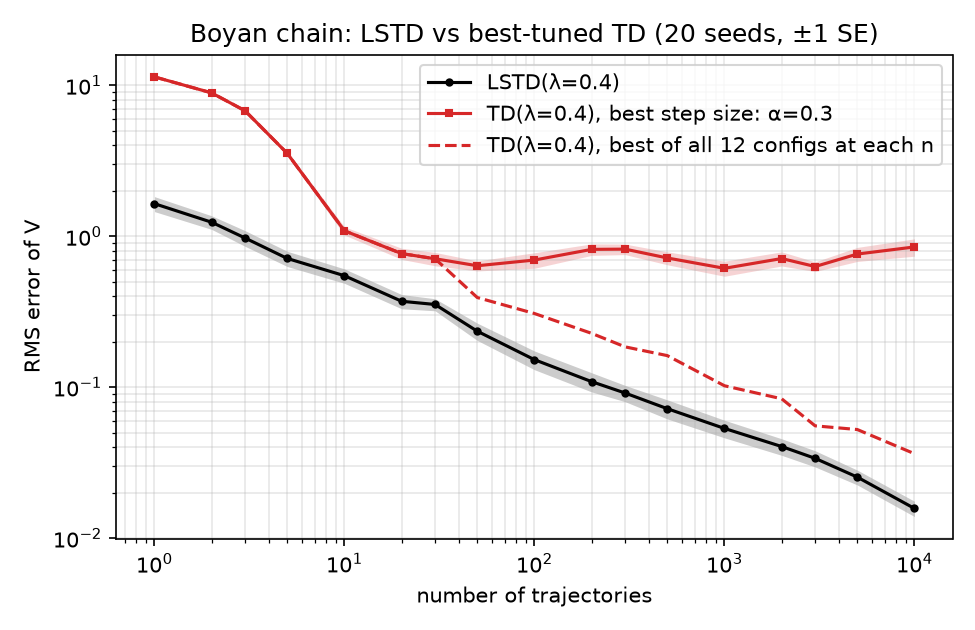
\includegraphics[width=\linewidth]{fig1_headline.png}
    \column{0.37\textwidth}
    \stat{1.64 $\to$ 0.016}{LSTD RMSE from 1 to $10^4$ trajectories}
    \stat{$\approx$\,0.7}{where the best single TD $\alpha$ (0.3) plateaus}
    \stat{$\approx$\,2$\times$}{lower error than \emph{oracle-tuned} TD (dashed) at every $n$}
    \stat{3--4$\times$}{fewer trajectories for the same error}
  \end{columns}
\end{frame}

\begin{frame}{Reproducing the paper's Figures 5 and 6}
  \speaker{\memberD}
  \begin{columns}[T]
    \column{0.5\textwidth}
    \centering
    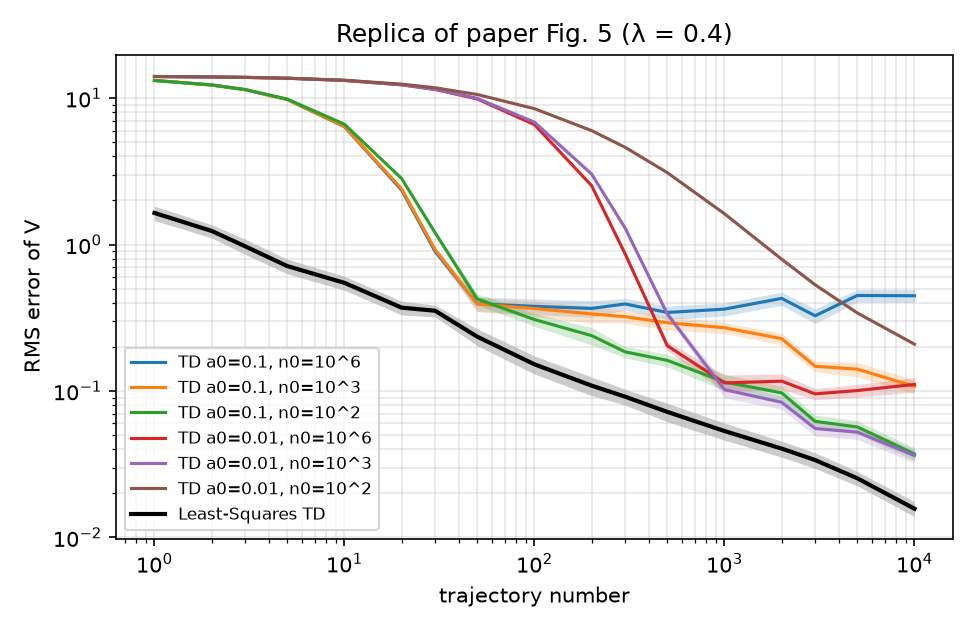
\includegraphics[width=\linewidth]{fig1b_paper_fig5.png}\\
    \small Paper Fig.~5: $\lambda = 0.4$, six schedules of Eq.~8
    \column{0.5\textwidth}
    \centering
    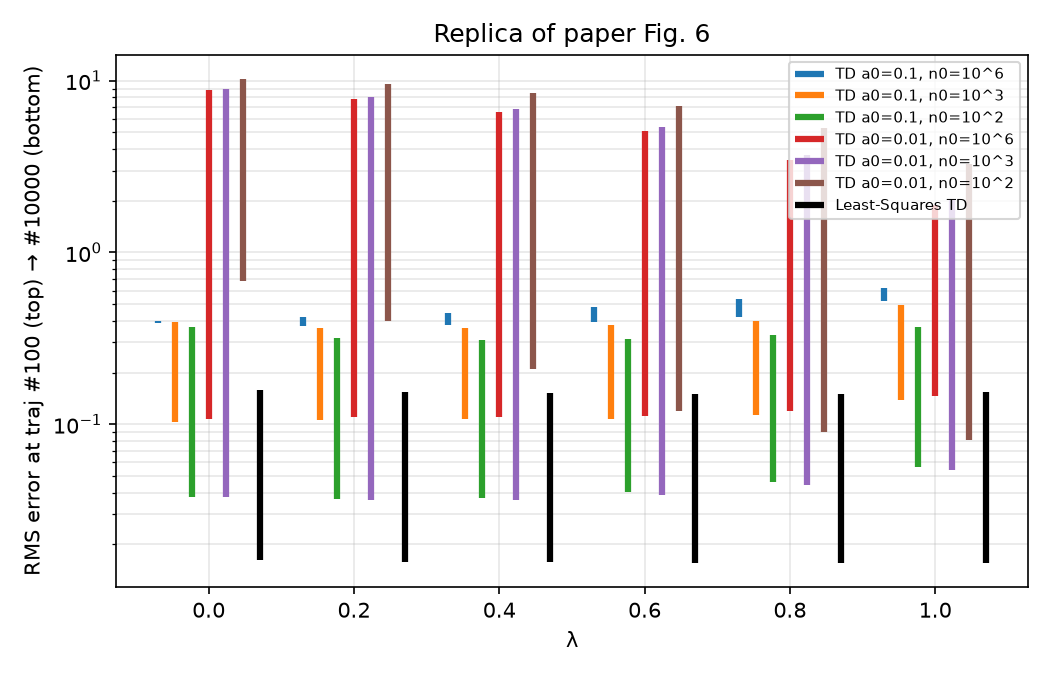
\includegraphics[width=\linewidth]{fig3b_paper_fig6.png}\\
    \small Paper Fig.~6: error at $n=100$ (top) $\to 10^4$ (bottom)
  \end{columns}
  \vspace{0.3em}
  \centering
  \hl{Same conclusion as the paper:} LSTD is best at every $\lambda$; TD depends critically on the schedule.
\end{frame}

\begin{frame}{Effect of $\lambda$}
  \speaker{\memberD}
  \begin{columns}[c]
    \column{0.5\textwidth}
    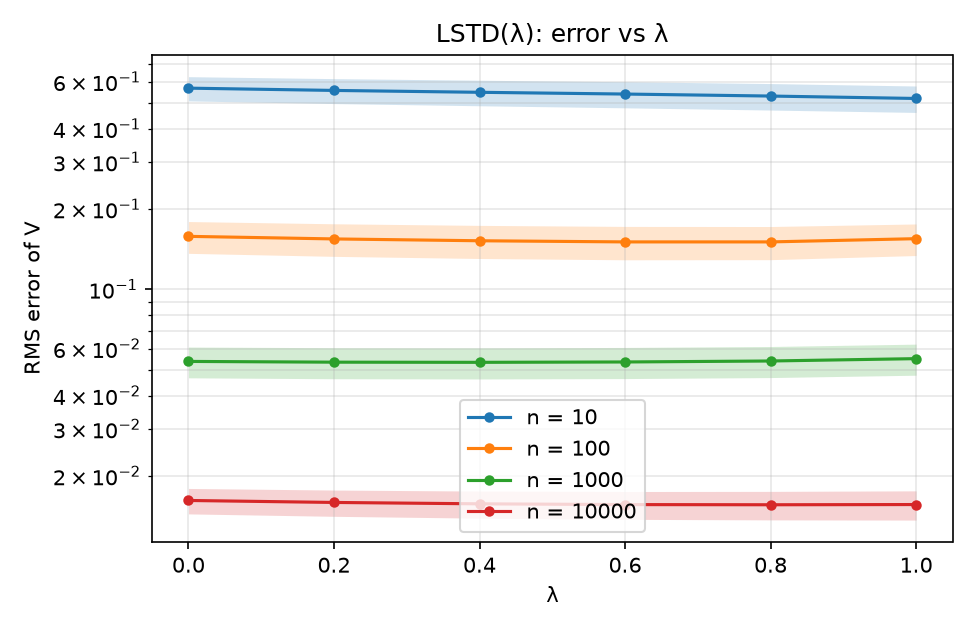
\includegraphics[width=\linewidth]{fig3_lstd_lambda.png}
    \column{0.48\textwidth}
    \small
    \begin{tabular}{@{}ccccc@{}}
      \toprule
      & \multicolumn{2}{c}{$n = 100$} & \multicolumn{2}{c}{$n = 10^4$} \\
      $\lambda$ & LSTD & TD$^\star$ & LSTD & TD$^\star$ \\
      \midrule
      0.0 & \textbf{0.158} & 0.368 & \textbf{0.016} & 0.038 \\
      0.2 & \textbf{0.155} & 0.318 & \textbf{0.016} & 0.036 \\
      0.4 & \textbf{0.152} & 0.308 & \textbf{0.016} & 0.036 \\
      0.6 & \textbf{0.151} & 0.312 & \textbf{0.016} & 0.039 \\
      0.8 & \textbf{0.151} & 0.329 & \textbf{0.016} & 0.044 \\
      1.0 & \textbf{0.155} & 0.366 & \textbf{0.016} & 0.054 \\
      \bottomrule
    \end{tabular}
    \vspace{0.3em}

    TD$^\star$ = best of 12 TD configs for that $n$ and $\lambda$.
    \begin{itemize}
      \item $\lambda$ barely matters for LSTD here (features are exact)
      \item LSTD beats oracle-tuned TD by $2$--$3.5\times$ everywhere
    \end{itemize}
  \end{columns}
\end{frame}

\begin{frame}{Novelty: ridge LSTD for very few trajectories}
  \speaker{\memberD}
  \begin{itemize}
    \item With 1--10 trajectories, $A$ can be singular or ill-conditioned $\Rightarrow$ $\vth = A^{-1}\mathbf{b}$ is unstable.
    \item \textbf{Ridge LSTD:}
      \[ (A + \epsilon I)\,\vth = \mathbf{b} \]
      (equivalently: recursive LSTD with $B_0 = I/\epsilon$).
    \item \textbf{Questions:}
      \begin{enumerate}
        \item How does the error depend on $\epsilon$ for $n \in \{1, 2, 5, 10\}$?
        \item Can a small $\epsilon$ make LSTD competitive with the best-tuned TD at 1--5 trajectories?
        \item What happens beyond the paper: \textbf{19-state random walk} (Sutton \& Barto) with \textbf{weak features} (5 aggregated groups, $V^\pi$ not representable)?
      \end{enumerate}
    \item 50 seeds, $\lambda = 0.4$, $\epsilon \in [10^{-4}, 10^2]$; TD reference = best of 5 constant $\alpha$ at each $n$.
  \end{itemize}
\end{frame}

\begin{frame}{Novelty: results}
  \speaker{\memberD}
  \begin{columns}[T]
    \column{0.5\textwidth}
    \centering
    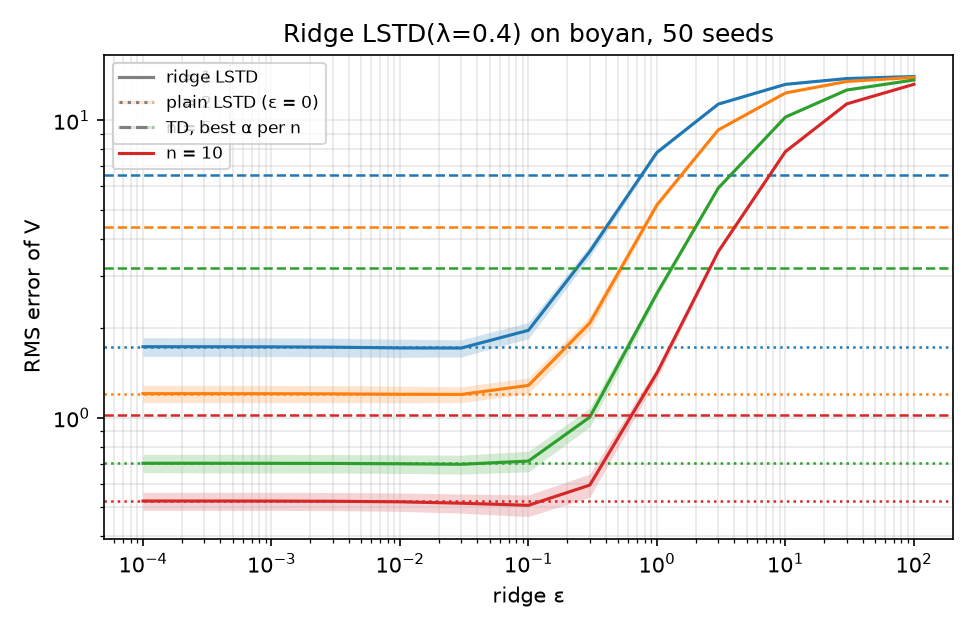
\includegraphics[width=\linewidth,height=4.3cm,keepaspectratio]{fig5_ridge_boyan.png}
    \column{0.5\textwidth}
    \centering
    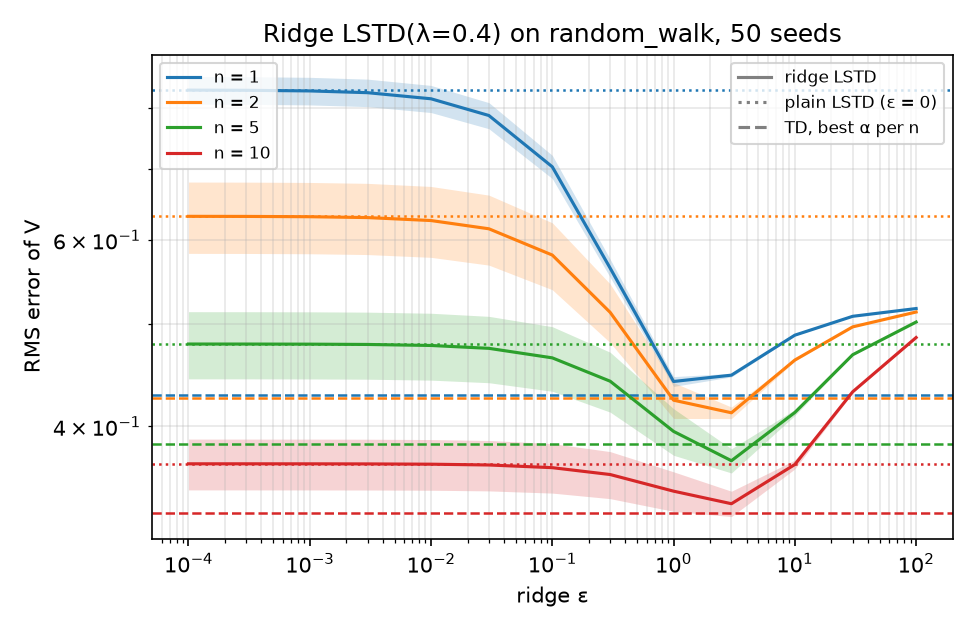
\includegraphics[width=\linewidth,height=4.3cm,keepaspectratio]{fig5_ridge_random_walk.png}
  \end{columns}
  \small
  \begin{columns}[T]
    \column{0.5\textwidth}
    \textbf{Boyan chain:} almost no gain (1--3\% at $\epsilon\approx0.03$). $A$ is already well conditioned; shrinking toward 0 hurts when $V$ is down to $-24$. Plain LSTD already beats TD (1.7 vs.\ 6.5 at $n=1$).
    \column{0.5\textwidth}
    \textbf{Random walk, weak features:} $\epsilon \approx 1$--3 \hl{halves the error at $n=1$} (0.83 $\to$ 0.44), matching best-tuned TD (0.43); slightly better than TD at $n = 2, 5$; TD marginally better at $n = 10$.
  \end{columns}
\end{frame}

\begin{frame}{Conclusions and limitations}
  \speaker{\memberD}
  \small
  \begin{columns}[T]
    \column{0.53\textwidth}
    \textbf{Conclusions}
    \begin{itemize}
      \item \hl{Reproduced the paper:} LSTD beats TD at every $n$, $\lambda$ and step size ($2$--$3.5\times$ below oracle-tuned TD).
      \item TD's best $\alpha$ depends on the data budget; a bad $\alpha$ costs $10$--$100\times$.
      \item LSTD: no step size, insensitive to $\lambda$ here.
      \item Price: $O(K^2)$ per step vs.\ $O(K)$.
      \item Ridge helps when data are scarce \emph{and} features weak.
    \end{itemize}
    \column{0.44\textwidth}
    \textbf{Limitations}
    \begin{itemize}
      \item Toy chains; Boyan features are exact (best case for LSTD).
      \item TD tuned over a 12-point grid only.
      \item Fixed $\epsilon$ weakens as $n$ grows ($A$ is a sum).
      \item Ridge shrinks toward $\vth = 0$, not a prior.
    \end{itemize}
  \end{columns}
  \begin{keyidea}
    \small\textbf{Next:}\enspace Mountain Car with tile coding (large $K$)\enspace\textperiodcentered\enspace
    LSPI: LSTD for control\enspace\textperiodcentered\enspace clipped / sign TD-error baselines
  \end{keyidea}
\end{frame}

\begin{frame}[plain]
  \begin{tikzpicture}[remember picture,overlay]
    \darkbg
    \node[anchor=south west,inner sep=0pt,text=white,font=\fontsize{40}{44}\selectfont\bfseries]
      at ([xshift=1.1cm,yshift=0.3cm]current page.west) {Thank you};
    \fill[accent] ([xshift=1.1cm,yshift=-0.15cm]current page.west) rectangle ++(1.4cm,0.09cm);
    \node[anchor=north west,inner sep=0pt,text=accent,font=\Large\bfseries]
      at ([xshift=1.1cm,yshift=-0.55cm]current page.west) {Questions?};
    \node[anchor=south west,inner sep=0pt,text=white!60!ink,font=\small]
      at ([xshift=1.1cm,yshift=0.75cm]current page.south west)
      {\faCode\enspace\texttt{src/}\qquad\faCheckCircle\enspace\texttt{tests/}\qquad\faChartLine\enspace\texttt{results/figures/}};
  \end{tikzpicture}
\end{frame}

% =========================================================================
\appendix
\backuptrue
\section*{Backup}

\begin{frame}{Backup: likely questions}
  \footnotesize
  \begin{description}[Why more data-efficient?]
    \item[Why more data-efficient?] It keeps every transition in $A$, $\mathbf{b}$ and solves exactly. TD uses each sample for one small step and then forgets it. LSTD is effectively model-based.
    \item[What if $A$ is singular?] Too little data or redundant features. Paper: SVD pseudo-inverse. Us: \texttt{solve} with SVD fallback, or ridge $(A+\epsilon I)$.
    \item[Cost in $K$?] $O(K^2)$ per step, $O(K^3)$ per solve (or $O(K^2)$ per step with recursive LSTD), vs.\ $O(K)$ for TD. Many features + cheap data $\Rightarrow$ TD can win on wall-clock time.
    \item[LSTD with $\lambda=1$?] Linear regression of features onto Monte-Carlo returns.
    \item[Control?] Yes: LSTD-Q inside policy iteration = LSPI (Lagoudakis \& Parr, 2003).
    \item[Is the comparison fair?] Same episodes per seed; TD gets its best of 12 configs at every $n$.
    \item[Why does ridge not help on Boyan?] $A$ is well conditioned, and shrinkage biases $\vth$ toward 0 while $\vth^* = (-24,-16,-8,0)$.
  \end{description}
\end{frame}

\begin{frame}{Backup: why LSTD(1) = Monte-Carlo regression}
  With $\lambda = \gamma = 1$, $\vz_t = \sum_{i\le t}\vphi_i$ and $\vphi_{T} = 0$ at termination:
  \[
    A = \sum_t \vz_t(\vphi_t - \vphi_{t+1})^\top
      = \sum_i \vphi_i \sum_{t\ge i}(\vphi_t - \vphi_{t+1})^\top
      = \sum_i \vphi_i\vphi_i^\top
  \]
  \[
    \mathbf{b} = \sum_t \vz_t r_t = \sum_i \vphi_i \sum_{t\ge i} r_t = \sum_i \vphi_i G_i
  \]
  So $\vth = A^{-1}\mathbf{b}$ is ordinary least squares of $G_i$ on $\vphi_i$ --- built incrementally without storing trajectories.
\end{frame}

\begin{frame}{Backup: code $\leftrightarrow$ paper}
  \small
  \begin{tabular}{@{}lll@{}}
    \toprule
    Paper & Code & Owner \\
    \midrule
    Fig.~4 chain and features & \texttt{env.BoyanChain}, \texttt{features.boyan\_features} & A \\
    Exact $V^\pi$ & \texttt{env.true\_values} (Bellman solve) & A \\
    Fig.~1 TD($\lambda$), Eq.~8 & \texttt{td\_lambda.td\_lambda\_curve}, \texttt{step\_size} & B \\
    Fig.~2 LSTD($\lambda$) & \texttt{lstd.lstd\_lambda\_curve}, \texttt{solve\_theta} & C \\
    Recursive LSTD (Sec.~2) & \texttt{lstd.recursive\_lstd} & C \\
    Sec.~3 model-based view & \texttt{tests/test\_lstd.py} & C \\
    Figs.~5, 6 and our figures & \texttt{run\_experiment.py}, \texttt{plot\_results.py} & D \\
    \bottomrule
  \end{tabular}
  \vspace{0.6em}

  \texttt{python -m src.run\_experiment \&\& python -m src.plot\_results}
\end{frame}

\end{document}
